%% Ankur Sinha

%% packages %%
% support for coloured text
\usepackage{color}
% IPA
\usepackage{tipa}
\usepackage[scale=2]{ccicons}
\usepackage{amssymb}
\usepackage{tikz}
\usetikzlibrary{mindmap, arrows.meta, positioning, arrows}
\usepackage{pgfplots}
% Define the colours we use for E and I in all graphs
\definecolor{SinhaBlueE}{HTML}{3b4cc0}
\definecolor{SinhaRedI}{HTML}{f7a789}
\pgfmathdeclarefunction{gaussnew}{4}{%nu, eta, eps, omega
  \pgfmathparse{(#1*((2*exp(-(((x-((#2+#3)/2))/((#2-#3)/(2*sqrt(-ln(#4/2)))))^2))) -#4))}%chktex 36
}
\usepackage{jneurosci}
\usepackage{subcaption}
\usepackage[T1]{fontenc}
\usepackage[utf8]{inputenc}
\usepackage[style=nature,backend=biber,autocite=footnote]{biblatex}
\addbibresource{/home/asinha/Documents/01_Readables/00_research_papers/bibliography/masterbib.bib}
% Use opensans
% \usepackage[default,scale=0.95]{opensans}
\usepackage[sfdefault]{roboto}
% for strike through
\usepackage[normalem]{ulem}
% links, urls, refs
\definecolor{links}{HTML}{2A1B81}
% Fedora blue for the theme
\definecolor{FedoraBlue}{HTML}{2A1B81}
\usepackage{hyperref}
\hypersetup{colorlinks,linkcolor=Green,urlcolor=links}
% graphics
\usepackage{graphicx}
% algorithm
\usepackage{algorithmic}
\usepackage{textcomp}
\usepackage{wrapfig}
\usepackage{textgreek}
\usepackage{euler}
\usepackage{csquotes}
\usepackage{tabularx}
\usepackage{booktabs}
% beamer theme
% use defaults for theme
\usetheme[numbering=fraction]{metropolis}
\usefonttheme[onlymath]{serif}
\setbeamerfont{footnote}{size=\tiny}
\setbeamerfont{caption}{size=\tiny}
\setbeamercolor{alerted text}{fg=Green}
\setbeamerfont{note page}{size=\small}

% Not needed in metropolis, but in general footnote citation fixes: https://tex.stackexchange.com/questions/44217/how-can-i-stop-footcite-from-hijacking-my-beamer-columns
% how to use multiple references to the same footnote: https://tex.stackexchange.com/questions/27763/beamer-multiple-references-to-the-same-footnote

% Disable footnoterule
\renewcommand{\footnoterule}{}

%% title %%
\title{Theory/modelling club!}
\subtitle{Structural plasticity and associative memory in balanced neural networks with spike-time dependent inhibitory plasticity}
\author[Ankur Sinha]{Ankur Sinha}
\date{02/06/2020}

%% document begins %%
\begin{document}


% title frame %%
\begin{frame}
  \titlepage{}
\end{frame}

%% Three slides for 5 minutes seems good
%% So, 30 slides at most for 50 minutes
\section{Context: what and why?}
\begin{frame}[c]{Peripheral lesions: large scale reorganisation in the brain}
  \begin{itemize}
    \item \fullcite{Rasmusson1982}
  \pause{}
  \scriptsize{
      \item \fullcite{Wall1984}
      \item \fullcite{Merzenich1984}
      \item \fullcite{Calford1988}
      \item \fullcite{Heinen1991}
      \item \fullcite{Rajan1993}
      }
  \end{itemize}
\end{frame}
\begin{frame}[c]{Imaging confirms structural plasticity in these experiments}
    \begin{itemize}
      \item \fullcite{DarianSmith1994}
        \pause{}
        \footnotesize{
      \item \fullcite{Florence1998}
      \item \fullcite{Keck2008}
      \item \fullcite{Keck2011}
      \item \fullcite{Marik2014}
      }
    \end{itemize}
\end{frame}
\begin{frame}[c]{Also confirms structural plasticity in the unlesioned adult brain}
    \begin{itemize}
      \item \fullcite{Holtmaat2005}
        \pause{}
        \footnotesize{
      \item \fullcite{Stettler2006}
      \item \fullcite{Marik2010}
      \item \fullcite{Chen2012}
      \item \fullcite{Villa2016}
      }
    \end{itemize}
\end{frame}
\begin{frame}[c]
  \frametitle{Example: Keck et al. 2008}
  \begin{figure}[h]
    \centering
    \includegraphics[width=0.8\linewidth]{99_images/keck-figure1}
  \end{figure}
  \footnotetext[1]{\fullcite{Keck2008}}
\end{frame}
\begin{frame}[c]
  \frametitle{Example: Keck et al. 2008: II}
  \begin{figure}[h]
    \centering
    \includegraphics[width=0.8\linewidth]{99_images/keck-figure2}
  \end{figure}
  \footnotetext[1]{\fullcite{Keck2008}}
\end{frame}
\begin{frame}[c]
  \frametitle{Features of repair}
  \input{table-strp-lit-review}
\end{frame}
\begin{frame}[c]
  \frametitle{Research question}
  How does repair by structural plasticity affect the function of the brain network?
\end{frame}
\section{How?}
\begin{frame}[c]
  \frametitle{Network dynamics during repair: Butz et al.}
  \begin{figure}[h]
    \centering
    \includegraphics[width=0.8\linewidth]{99_images/butz3.png}
  \end{figure}
  \footnotetext[2]{\fullcite{Butz2013}}
\end{frame}
\begin{frame}[c]
  \frametitle{Butz2013: activity dependent homeostatic structural plasticity}
  \begin{columns}
    \begin{column}{0.5\textwidth}
      \begin{figure}[h]
        \centering
        \includegraphics[width=0.8\linewidth]{99_images/neurons-strp}
      \end{figure}
    \end{column}
    \begin{column}{0.5\textwidth}
      \begin{figure}[h]
        \centering
        \includegraphics[width=0.8\linewidth]{99_images/growth-curve-general}
      \end{figure}
    \end{column}
  \end{columns}
  \footnotetext[2]{\fullcite{Butz2013}}
\end{frame}
\begin{frame}[c]
  \frametitle{Butz2013: activity dependent homeostatic structural plasticity}
  \begin{columns}
    \begin{column}{0.5\textwidth}
      \begin{figure}[h]
        \centering
        \includegraphics[width=0.8\linewidth]{99_images/lipton1989}
      \end{figure}
    \end{column}
    \begin{column}{0.5\textwidth}
      \begin{figure}[h]
        \centering
        \includegraphics[width=0.8\linewidth]{99_images/growth-curve-general}
      \end{figure}
    \end{column}
  \end{columns}
  \footnotetext[2]{\fullcite{Butz2013}}
  \footnotetext[3]{\fullcite{Lipton1989}}
\end{frame}
\begin{frame}[c]
  \frametitle{Re-implementation/investigation of Butz et al.'s model}
  \input{table-butz-results}
\end{frame}
\begin{frame}[c]
  \frametitle{Proxy for network function: associative memory storage}
  \begin{figure}[h]
    \centering
    \includegraphics[width=\linewidth]{99_images/vogels-figure4}
  \end{figure}
  \footnotetext[4]{\fullcite{Vogels2011}}
\end{frame}
\begin{frame}[c]
  \frametitle{Re-implementation/verification of associative memory model}
  \begin{figure}[htpb]
  \begin{subfigure}[h]{0.3\textwidth}
    \resizebox{1.2\textwidth}{!}{\input{99_images/B-ratematrix.tex}}
  \end{subfigure}
  \begin{subfigure}[h]{0.3\textwidth}
    \resizebox{1.2\textwidth}{!}{\input{99_images/C-ratematrix.tex}}
  \end{subfigure}
  \begin{subfigure}[c]{0.3\textwidth}
    \resizebox{1.2\textwidth}{!}{\input{99_images/D-ratematrix.tex}}
  \end{subfigure}
  \end{figure}
\end{frame}
\begin{frame}[c]
  \frametitle{Expected research path}
  Apply Butz et al.'s model of structural plasticity to the Vogels-Sprekeler's cortical model, store associative memories, measure performance before, during, after repair.
\end{frame}
\begin{frame}[c]
  \frametitle{Model schematic}
  \begin{figure}[h]
    \centering
    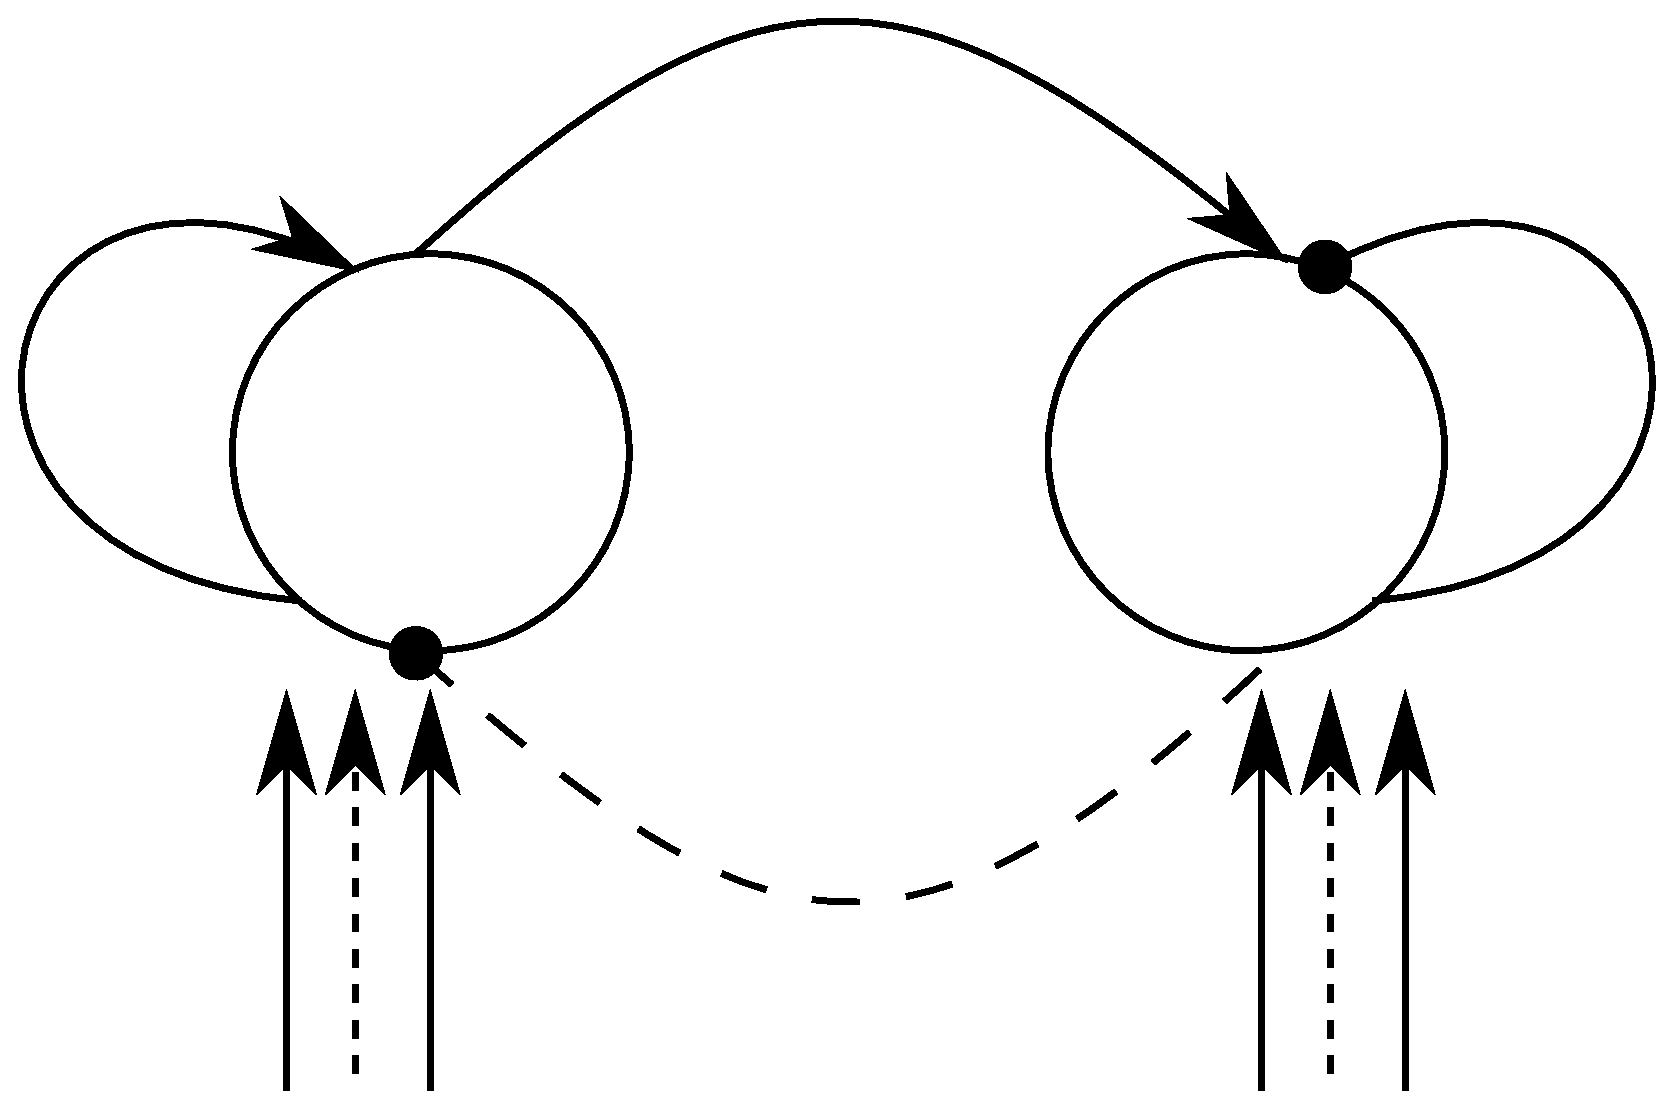
\includegraphics[width=0.8\linewidth]{99_images/schematic}
  \end{figure}
\end{frame}
\begin{frame}[c]
  \frametitle{Simulation protocol}
  \begin{figure}[h]
    \centering
    \includegraphics[width=0.8\linewidth]{99_images/recall-protocol}
  \end{figure}
\end{frame}
\begin{frame}[c]
  \frametitle{Effect of deafferentation on cortical model}
  \begin{figure}[h]
    \centering
    \includegraphics[width=0.5\linewidth]{99_images/deaff-only}
  \end{figure}
\end{frame}
\begin{frame}[c]
  \frametitle{Rejection of Butz et al.'s growth curve hypothesis}
  If Butz et al.'s single growth curve for all neurites is correct, the increase in activity outside the LPZ  as a result of deafferentation will cause:
  \begin{itemize}
    \item retraction of excitatory pre-synaptic elements outside the LPZ,
    \item retraction of inhibitory post-synaptic elements outside the LPZ\@.
  \end{itemize}
\end{frame}
\section{Results}
\begin{frame}[c]
  \frametitle{New model of peripheral lesioning and repair in cortical network}
  \begin{figure}[h]
    \centering
    \includegraphics[width=0.5\linewidth]{99_images/deaff-repair}
  \end{figure}
  \footnotetext[5]{\fullcite{Sinha2019}}
\end{frame}
\begin{frame}[c]
  \frametitle{New growth curves for post-synaptic neurites}
  \begin{figure}[h]
    \centering
    \includegraphics[width=0.6\linewidth]{99_images/growth-post}
  \end{figure}
\end{frame}
\begin{frame}[c]
  \frametitle{Stabilisation of individual neurons}
  \begin{figure}[h]
    \centering
    \includegraphics[width=0.4\linewidth]{99_images/single-neuron-results}
  \end{figure}
\end{frame}
\begin{frame}[c]
  \frametitle{New growth curves for pre-synaptic neurites}
  \begin{figure}[h]
  \begin{subfigure}[h]{0.4\textwidth}
    \includegraphics[width=\textwidth]{99_images/possible-growth-pre}
  \end{subfigure}
  \begin{subfigure}[c]{0.5\textwidth}
    \includegraphics[width=\textwidth]{99_images/growth-pre-table.png}
  \end{subfigure}
  \end{figure}
\end{frame}
\begin{frame}[c]
  \frametitle{New growth curves for pre-synaptic neurites}
  \begin{figure}[h]
    \centering
    \includegraphics[width=0.6\linewidth]{99_images/growth-pre}
  \end{figure}
\end{frame}
\begin{frame}[c]
  \frametitle{Both synaptic and structural plasticity are necessary for repair}
  \begin{figure}[h]
    \centering
    \includegraphics[width=0.6\linewidth]{99_images/syn-str-both}
  \end{figure}
\end{frame}
\begin{frame}[c]
  \frametitle{Associative memory performance after deafferentation (no repair)}
  \begin{figure}[h]
    \centering
    \includegraphics[width=0.6\linewidth]{99_images/performance-deaff-only}
  \end{figure}
\end{frame}
\begin{frame}[c]
  \frametitle{Associative memory performance during repair}
  \begin{figure}[h]
    \centering
    \includegraphics[width=0.6\linewidth]{99_images/performance-during-repair}
  \end{figure}
\end{frame}
\end{document}

